\chapter{Combat}\label{Combat}
    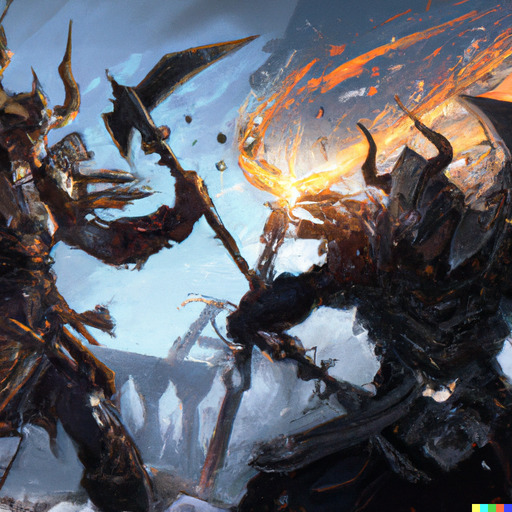
\includegraphics[width=\columnwidth]{combat/combat}
    The world of Rise can be a harsh one, and not all disagreements can be resolved peacefully.
    At some point, you will be forced to enter combat.
    This chapter explains how combat works in Rise.

\section{Making Attacks}\label{Attacks}
    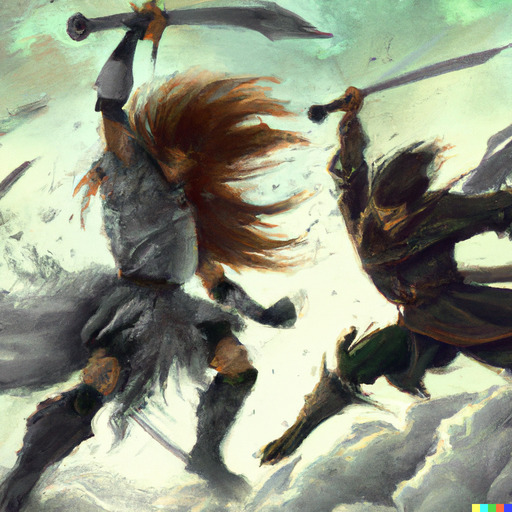
\includegraphics[width=\columnwidth]{core mechanics/making attacks}

    \subsection{Attack Rolls}\label{Attack Rolls}
        To make an attack, roll 1d10 and add your \glossterm{accuracy} with the attack.
        Each attack specifies a relevant \glossterm{defense} (see \pcref{Defenses}).

        If the result of your attack roll meets or exceeds the defense of the creature or object you are attacking, the attack hits.
        If your result is 1 or 2 lower than the defender's defense, you get a \glossterm{glancing blow} (see below).
        Otherwise, the attack misses.

        \subsubsection{Glancing Blows}\label{Glancing Blows}
            When you miss on an attack by 2 or less, it is called a \glossterm{glancing blow}.
            All damaging attacks have a standard glancing blow effect.
            If you get a glancing blow with a damaging attack, you roll no damage dice.
            However, if the attack deals damage that is not based on dice, you still deal that damage.
            For example, many attacks add your \glossterm{power} to damage, and that damage is still dealt on a glancing blow.

            Non-damaging attacks do not have any special effects on a glancing blow.
            A glancing blow is not considered to be a miss for the purpose of abilities that trigger on missed attacks.
            However, many abilities trigger on both glancing blows and missed attacks, such as a \mitem{hardblock shield}.

        \subsubsection{Exploding Attacks}\label{Exploding Attacks}
            When you make an attack roll, if you roll a 10 on the d10, the die \glossterm{explodes}.
            In addition, some effects can cause your roll to \glossterm{explode} without rolling a 10.

            When an attack roll \glossterm{explodes}, you roll it again and add the second result to the original result before applying your \glossterm{accuracy}.
            If you roll a 10 on the extra roll, you keep rolling until you stop rolling a 10 and add all of the rolls together.

        \subsubsection{Critical Hits}\label{Critical Hits}
            If your attack result is at least 10 higher than your target's defense, your attack is a \glossterm{critical hit}.
            Some attacks have specific effects when you get a critical hit.
            In addition, all damaging attacks have a standard critical hit effect.
            For every increment of 10 by which you beat the target's defense, you double the number of damage dice you roll.
            As normal, two doublings become a tripling, so if you beat your opponent's defense by 20, you roll triple the damage dice.
            This does not increase the damage from your \glossterm{power} or any other non-dice damage modifiers.

            Objects are not normally subject to critical hits.
            Some creatures are also not subject to critical hits, as noted in their descriptions.

            Critical hits with \glossterm{melee} attacks are a \abilitytag{Size-Based} effect.
            This means you cannot normally get a critical hit with a melee attack against a creature that is two or more size categories larger than you (see \pcref{Size Categories}).

    \subsection{Dealing Damage}\label{Dealing Damage}
        Many \glossterm{attacks} deal damage to their targets.
        When a creature is dealt damage, it gets closer to death (see \pcref{Taking Damage}).
        In general, most damaging attacks deal an amount of damage determined by rolling some number of dice and adding some multiplier of your \glossterm{power} with that attack.
        The details are given in each attack's description.

        \subsubsection{Dice Pools}\label{Dice Pools}
            Almost all attacks deal damage based on a \glossterm{dice pool}.
            Likewise, healing abilities usually heal hit points based on a dice pool.
            Dice pools are written with the number of dice, followed by ``d'', followed by the size of dice to roll.
            For example, 2d6 means you roll two six-sided dice.
            You always sum the roll of all dice rolled in a dice pool to determine the total result.

            Some modifiers add or subtract flat values from the result of the dice pool.
            Others add or subtract \glossterm{dice increments}.

            A die increment is a single increase or decrease in the value of a dice pool.
            Increasing by one die increment is written as \plus1d, and decreasing by one die increment is written as \minus1d.
            Damage dice change in size according to the following pattern:
            \begin{itemize}
                \item 1 damage (minimum)
                \item 1d2
                \item 1d3
                \item 1d4
                \item 1d6
                \item 1d8
                \item 1d10
                \item 2d6
                \item 2d8
                \item 2d10
                \item 4d6
                \item 4d8
                \item 4d10
                \item 5d10
                \item 6d10
                \item 7d10
                \item 8d10
            \end{itemize}

            For each die increment that increases the damage, move one space down the list.
            Likewise, for each die increment that decreases the damage, move one space up the list.
            After the dice pool reaches 8d10, each additional die increment adds an additional 1d10.
            In practice, you are unlikely to ever roll that many dice.

            \parhead{Dice Bonuses From Attributes}\label{Dice Bonuses From Attributes} Your attributes can add or subtract dice increments from all dice pools you roll.
            Whenever you use a \glossterm{mundane} ability that has a dice pool, you add half your Strength in dice increments to the dice pool.
            If your Strength is negative, this can reduce your damage or healing.
            Likewise, you add half your Willpower in dice increments to your dice pools with \glossterm{magical} abilities.
            For example, if you are using a spell that normally deals 1d8 damage, and your Willpower is 2 or 3, you would deal 1d10 damage with that ability instead.

            Items are an exception to this rule.
            Some items specify their own dice pools, like a \mitem{firebomb} or a \mitem{vampiric} weapon.
            Your Strength and Willpower do not modify the dice pools specified by items.

    % TODO: different section?
    \subsection{Damage Types}\label{Damage Types}
        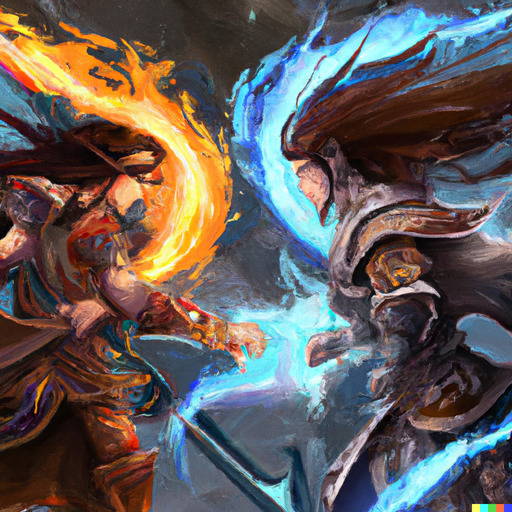
\includegraphics[width=\columnwidth]{core mechanics/damage types}
        Almost all damage falls into one of two categories: \glossterm{energy damage} or \glossterm{physical damage}.
        Physical damage is the most common type of damage.
        Energy damage is usually caused by \glossterm{magical} effects.

        A rare few effects deal damage that has no type.
        Poisons are the most common way to deal untyped damage.
        Untyped damage has no special properties, but effects that help you specifically resist energy damage or physical damage do not help against untyped damage.

        \subsubsection{Damage Subtypes}\label{Damage Subtypes}
            Physical damage has four subtypes: acid damage, bludgeoning damage, piercing damage, and slashing damage.
            Energy damage has four subtypes: cold damage, electricity damage, fire damage, and psychic damage.
            Damage of a particular subtype is also considered damage of its primary type.
            For example, if you are \trait{impervious} to \glossterm{physical damage}, that applies against bludgeoning damage because bludgeoning damage is a subtype of \glossterm{physical damage}.

            Some damage types have special properties, as described below.
            \parhead{Cold} Abilities that deal cold damage can freeze liquids and have similar effects appropriate to a sudden drop in temperature.
            \parhead{Electricity} Abilities that deal electricity damage can ignite nonmagical fires if they damage combustible objects.
            \parhead{Fire} Abilities that deal fire damage provide light equivalent to a torch for their duration.
            % TODO: what does this actually mean
            Abilities without a duration create a brief burst of torchlight.
            While underwater, they deal half damage and have no nondamaging effects.

        \subsubsection{Multiple Damage Types}\label{Multiple Damage Types}
            Some attacks deal damage that has multiple damage types.
            Defensive abilities such as defense bonuses or damage immunities apply against an attack only if they apply to all damage types dealt by the attack.

    \subsubsection{Special Damage Types}\label{Special Damage Types}

        Subdual damage and environmental damage are separate from the standard damage types, like fire damage or energy damage.
        It is possible for damage to be both environmental damage and subdual damage.

        \subsubsection{Environmental Damage}\label{Environmental Damage}
            Some abilities and environmental effects deal environmental damage.
            Environmental damage is never dealt as the result of a successful attack roll.
            Environmental damage works in the same way as normal damage, except that environmental damage is reduced by your \glossterm{damage resistance} without subtracting from its remaining value.
            Any environmental damage in excess of a creature's damage resistance is causes the creature to lose hit points just like normal damage.

        \subsubsection{Subdual Damage}\label{Subdual Damage}
            Some attacks and environmental effects deal subdual damage.
            Subdual damage works in the same way as normal damage, except it cannot inflict \glossterm{vital wounds}.
            If an attack that deals subdual damage would inflict a vital wound, the target increases its \glossterm{fatigue level} by three instead.
            Whenever you make a \glossterm{strike}, you can choose to deal subdual damage instead of normal damage.
            If you do, you deal half damage with the strike.

\section{Taking Damage}\label{Taking Damage}
    Taking damage from attacks reduces your \glossterm{damage resistance}, and then your \glossterm{hit points}, before finally inflicting \glossterm{vital wounds}.
    To calculate your damage resistance and hit points, see \pcref{Character Statistics}.
    This section explains those concepts in more detail.

    When you are dealt damage, the damage first reduces your \glossterm{damage resistance} (see \pcref{Damage Resistance}).
    Any damage in excess of your remaining damage resistance causes you to lose that many \glossterm{hit points} (see \pcref{Hit Points}).
    Hit points and damage resistance function in the same way, but damage resistance can protect you from debilitating attacks that only work if they make you lose hit points.
    If you are dealt damage that reduces your hit points below 0, you gain one or more \glossterm{vital wounds} (see \pcref{Negative Hit Points}).

    Monsters typically do not gain vital wounds like player characters do.
    Instead, they simply die or fall unconscious when they reach 0 hit points.

    \subsection{Negative Hit Points}\label{Negative Hit Points}
        You can have negative hit points, but only briefly.
        When your hit points drop below 0, you gain a \glossterm{vital wound} (see \pcref{Vital Wounds}).
        You gain an additional vital wound for each increment of half your maximum hit points that you reach in negative hit points.
        If you heal past this threshold and then pass it again, you do not gain an extra vital wound.

        At the end of each round, if your hit points are negative, your hit points are reset to 0.
        This is checked after applying all healing and damage that takes place at the end of the round.
        This also resets the vital wound thresholds that you have suffered, so you will immediately suffer a vital wound if your hit points go negative again.

\section{Vital Wounds}\label{Vital Wounds}
    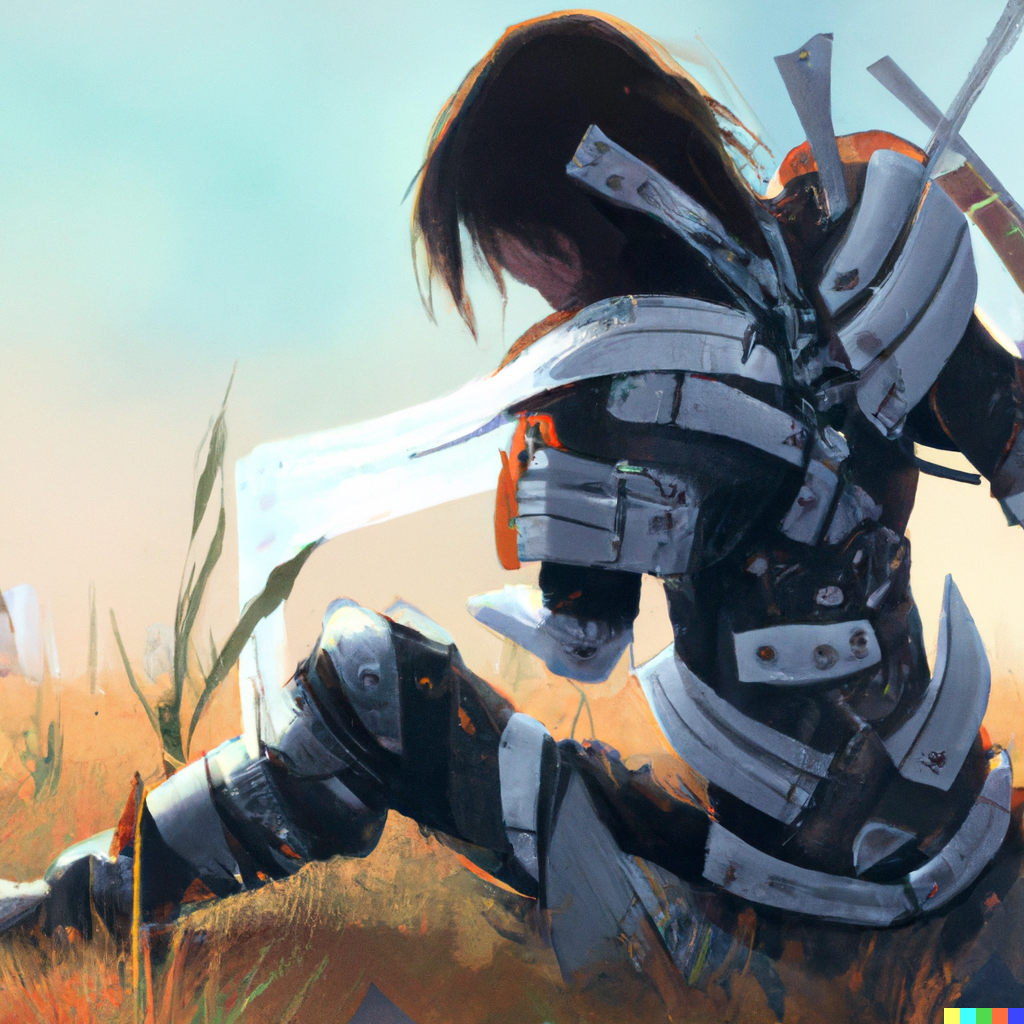
\includegraphics[width=\columnwidth]{core mechanics/vital wounds}

    A \glossterm{vital wound} represents serious damage to your body.
    Each \glossterm{vital wound} has a specific detrimental effect on you.
    You gain vital wounds when your \glossterm{hit points} go negative (see \pcref{Negative Hit Points}).

    To determine the effect of a \glossterm{vital wound}, make a \glossterm{vital roll} and find the corresponding effect in \trefnp{Vital Wound Effects}.
    The effect of the vital wound lasts until you remove that vital wound.
    The effects of vital wounds stack with each other, even if you roll the same effect twice for different \glossterm{vital wounds}.

    \subsection{Vital Rolls}\label{Vital Rolls}
        To make a \glossterm{vital roll}, roll 1d10.
        You take a penalty to this roll equal to twice the number of \glossterm{vital wounds} you already have, not counting the vital wound you are rolling for.
        This includes vital wounds that have no specific vital wound effect.
        The result determines the effect of the \glossterm{vital wound}, as listed in \tref{Vital Wound Effects}.
        Vital wound effects from vital rolls below 1 are lethal if untreated, but the Medicine skill can be used to prevent you from dying (see \pcref{Medicine}).
        This roll is not a \glossterm{check}, so you can't affect it with abilities like \glossterm{desperate exertion}.

        \parhead{Delaying Death} Vital wounds with a vital roll below 1 can kill you.
        While you are dying in this way, if you receive healing that causes you to regain hit points, you delay your death by one round.
        This benefit applies even if you are already at full hit points.
        You cannot delay your death in this way by more than 5 rounds.

        \begin{dtable}
            \lcaption{Vital Wound Effects}
            \begin{dtabularx}{\textwidth}{l X}
                \tb{Vital Roll}  & \tb{Effect} \tableheaderrule
                \minus6 or less  & You immediately die                                                    \\
                \minus1--\minus5 & You are unconscious, and you die at the end of the next round          \\
                0                & You are unconscious, and you die after one minute                      \\
                1                & You are unconscious while you have less than full hit points           \\
                2                & You have a \minus10 foot penalty to your speed with all movement modes \\
                3                & You have a \minus5 foot penalty to your speed with all movement modes  \\
                4                & You take a \minus2 penalty to all \glossterm{defenses}                 \\
                5                & You take a \minus1 penalty to all \glossterm{defenses}                 \\
                6                & Your maximum \glossterm{damage resistance} is 0                        \\
                7                & Your maximum \glossterm{damage resistance} is halved                   \\
                8                & You take a \minus2 penalty to \glossterm{accuracy}                     \\
                9                & You take a \minus1 penalty to \glossterm{accuracy}                     \\
                10 or more       & No extra vital wound effect                                            \\
            \end{dtabularx}
        \end{dtable}

    \subsection{Removing Vital Wounds}\label{Removing Vital Wounds}
        Vital wounds take time to heal.
        Whenever you take a \glossterm{long rest}, you remove one of your vital wounds.
        If you have multiple vital wounds, you may choose the order in which your vital wounds are removed.

\section{Combat Time}\label{Combat Time}
    This section explains how time passes in combat.

    \subsection{Rounds}\label{Rounds}

        Combat takes place in a series of \glossterm{rounds}, which represent about six seconds of time.
        Each round of a combat is divided into two \glossterm{phases}: the movement phase and the action phase (see \pcref{Phases}).
        After both phases are complete, the round ends and the next round begins.

    \subsection{Actions}\label{Actions}

        You can take actions in combat to defeat your foes.
        There are three types of actions: \glossterm{standard actions}, \glossterm{minor actions}, and \glossterm{free actions}.
        In addition, you can use \glossterm{movement} during the \glossterm{movement phase} (see \pcref{Movement and Positioning}).
        % TODO: define conflicting action limits (drawing a sword and sheathing a shield?)

        \subsubsection{Standard Actions}\label{Standard Actions}
            Most common activities require a \glossterm{standard action}, such as attacking with a weapon, casting a \glossterm{spell}, and using many special abilities.
            Using a standard action generally takes about three seconds of time within the game, and it requires most of your attention during that time.

            You can take one standard action during the \glossterm{action phase} of each round.

        \subsubsection{Minor Actions}\label{Minor Actions}
            Some special abilities require a \glossterm{minor action}.
            Using a minor action does not take much time or attention, and it can be done at the same time as any other actions.
            You cannot use a \glossterm{minor action} during the \glossterm{movement phase}.

            You can take one minor action during the \glossterm{action phase} of each round.
            In addition, you can choose to replace your standard action during the action phase with an additional minor action.
            However, you cannot use the same minor action twice in a single round unless an ability specifies otherwise.

        \subsubsection{Free Actions}\label{Free Actions}
            Some activities that take little time or attention require a \glossterm{free action}.
            You can take any number of free actions per round.
            However, you cannot use the same free action twice in a single round unless an ability specifies otherwise.
            This restriction is intended to limit the power of specific special abilities that require a free action to use.
            At the GM's discretion, you may take the same simple free action multiple times, such as dropping multiple objects in a single turn.

    \subsection{Phases}\label{Phases}

        There are two \glossterm{phases} in each round: a \glossterm{movement phase} and an \glossterm{action phase}.
        Each phase specifies the types of actions that can be taken during that phase.
        As a special case, \glossterm{free actions} may be taken during any phase.

        \subsubsection{The Movement Phase}\label{The Movement Phase}
            During the \glossterm{movement phase}, you can make one \glossterm{movement}.
            The most common movement is the \textit{hustle} ability, which allows you to move a distance equal to your \glossterm{speed}.
            For details, see \pcref{Movement and Positioning}.

        \subsubsection{The Action Phase}\label{The Action Phase}
            During the \glossterm{action phase}, you can take one \glossterm{minor action} and one \glossterm{standard action}.
            Alternately, you can make a \glossterm{movement} or take an additional \glossterm{minor action} in place of your standard action.
            Most of the time, you will simply take a single standard action.

    \subsection{Resolving Actions}\label{Resolving Actions}

        Actions in combat are partially sequential, and partially simultaneous.
        You and your \glossterm{allies} who can see or otherwise communicate with each other generally act as a single allied group.
        One at a time, each person in the allied group declares their actions, rolls all relevant dice, and applies the results appropriately.
        You can freely choose the order in which people act within the allied group, as long as everyone agrees with the order chosen.
        If one of your allies acts before you, you can learn the result of their action before deciding your own action.
        For example, if they knock an enemy \prone, that enemy would suffer the appropriate defense penalties against your attacks.

        Although your actions resolve sequentially within your allied group, they resolve simultaneously with the actions of anyone outside your allied group.
        Essentially, you locally resolve the effects of your actions within your allied group, but those actions do not globally resolve until later.
        This means that you cannot interrupt enemy actions, even by killing them.
        Generally, you won't know what actions your enemies will take until after you have already resolved your action.
        However, their actions will resolve as if they had acted before you, not after you.
        This goes both ways, of course.
        You can freely decide your actions without knowing what your enemy is doing because their actions cannot interrupt yours.

        Once all allied groups have locally resolved their actions, the results of all of those actions is announced.
        Then, each allied group updates their own status to reflect the actions that all of the other allied groups took during the same phase.
        In addition, any effects that automatically trigger during the action phase are resolved now.
        Once all of the actions have been globally resolved, the phase ends.
        In a typical combat, this just means that the GM will tell you what the monsters did to you after you tell the GM what you did to them.

        With this system, it's possible for two combatants to kill each other during the same phase, leaving both dead!
        This might seem strange if you're used to other games which always resolve one action at a time.
        However, this situation is not uncommon in fantasty fiction, and it's certainly possible in real life.

        \subsubsection{Delayed and Repeated Effects}
            Some abilities cause additional attacks or effects ``during your next action'' or ``during each of your subsequent actions''.
            Your action happens when you take your turn during the \glossterm{action phase}.
            You can choose when those effects happen during that turn.
            Typically, you would resolve them first so you know their results, but you can do that after your other actions if you want.
            You can't split those automatic effects from your other actions in the turn order, just like you can't take your \glossterm{minor action} separately from your \glossterm{standard action}.

        \subsubsection{Swift Abilities}\label{Swift Abilities}
            A small number of abilities with the \abilitytag{Swift} tag resolve differently from most actions.
            Swift abilities resolve before all non-Swift abilities, so they can change the results of your enemy's actions.
            However, Swift abilities are always simple, and cannot interrupt actions or make attack rolls.
            Generally, they simply increase or decrease a creature's defenses during the current round.
            You declare Swift abilities during your normal turn within your allied group, and you don't have to go first within your group or do anything special to use them.

            For example, the \ability{total defense} ability gives you a bonus to your defenses during the current phase.
            That ability has to resolve before your enemies attack you during that phase, or else it would be pointless.
            Some abilities have only part of their effect resolve early.
            For example, the \textit{reckless attack} ability immediately reduces your defenses, which affects attacks made against you during the current phase, and makes a \glossterm{strike} with the normal timing.

        \subsubsection{Action Resolution Summary} 
            \begin{enumerate*}
                \item Round begins - "start of round" resolve globally
                \item Movement phase begins - "start of phase" effects resolve globally
                \item Movements resolve globally, using \glossterm{initiative} checks when strictly necessary
                \item Movement phase ends - "end of phase" effects resolve globally
                \item Action phase begins - "start of phase" effects resolve globally
                \item \abilitytag{Swift} abilities resolve globally
                \item Actions of your allied group resolve locally
                \item Actions of other allied groups resolve locally
                \item Actions of each allied group are announced, and resolve globally
                \item Action phase ends - "end of phase" effects resolve globally
                \item Round ends - "end of round" effects resolve globally
            \end{enumerate*}

        \subsubsection{Deciding Action Order}\label{Deciding Action Order}
            Try not to spend too much time the exact order of everyone's actions within your allied group.
            Most of the time, the exact order doesn't matter.
            It's generally fine to just start rolling dice if you already know what you're going to do, and just act in the order that people decide their actions.
            The GM can help resolve situations where this is ambiguous.

        \subsubsection{Multi-Group Battles}\label{Multi-Group Battles}
            Sometimes, there might be more than two groups in a battle.
            This works in basically the same way as a two-sided battle.
            Each allied group resolves sequentially with itself, but simultaneously with all enemy groups.
            It's possible for two different groups to attack and kill the same creature, which wastes some of their actions.
            That's a natural consequence of not coordinating effectively.

        \subsection{Simultaneous Damage and Healing}\label{Simultaneous Damage and Healing}
            Most healing abilities are used as a standard action and resolve locally before you take any incoming damage.
            However, some abilities cause you to automatically recover hit points or damage resistance at specific times, like at the end of the round, when you can also take damage.
            If you regain hit points or damage resistance and take damage simultaneously, apply all damaging effects before applying any healing effects.

    % This may be too complicated
    \subsection{Conflicting Actions}\label{Conflicting Actions}
        Sometimes, actions that occur in the same phase can be mutually impossible.
        Almost all conflicting actions are the result of competing movements.
        When actions conflict, each creature involved rolls an \glossterm{initiative} check (see \pcref{Initiative}).
        Starting from the highest check result and continuing to the lowest, each creature immediately resolves its chosen action.
        Creatures that resolve their action afterward accomplish as much of their intended action as possible before being blocked or otherwise prevented.

        For example, if three different creatures attempt to move into the same space, only the creature with the highest initiative check would actually enter that space.
        The other two creatures would take their intended path, but they would interrupt their movement when they cannot proceed farther, generally because they run into the space occupied by the first creature.

        In general, directly conflicting actions are rare.
        Most movements do not conflict - even reactive movements, such as when one creature attempts to follow a withdrawing creature.
        In that case, no initiative check is necessary.
        Both creatures simply move as far as they can, and the creatures' relative movement speeds determine who is more successful.

        This does make it possible for creatures to be ``stranded'' out of melee range of any attackers.
        Player characters are normally allowed to break this symmetry by reactively using the \textit{sprint} ability, while monsters cannot sprint.
        This can help prevents melee characters from feeling stuck or useless.
        In addition, the \ability{charge} universal ability can be helpful in such cases.

        \subsubsection{Initiative}\label{Initiative}
            When multiple creatures take mutually impossible actions simultaneously, such as racing to be the first one to a door, they must roll an \glossterm{opposed check} with their initiative modifier.
            For details, see \pcref{Conflicting Actions}.
            Your initiative modifier is equal to your movement speed that you are using to take the action.
            In the unusual situation that no movement speed is relevant, just roll without applying a modifier.

\section{Movement and Positioning}\label{Movement and Positioning}
    This section describes how creatures move and position themselves on a battlefield.

    \subsection{Movements}\label{Movements}
        Abilities that require a movement typically move you around the battlefield, and are usually used in the \glossterm{movement phase}.
        Making a movement generally takes about three seconds of time within the game, and it requires most of your attention during that time.

        You can make one movement during the \glossterm{movement phase} of each round.
        In addition, you can choose to replace your standard action during the action phase with an additional movement.

    \subsection{Movement Modes}\label{Movement Modes}
        A \glossterm{movement mode} is a method of moving from one location to another.
        % TODO: terminology confusion mode vs. speed
        The most common movement mode is a land speed, which allows creatures to move across the ground.
        Unless otherwise noted, all creatures have a land speed equal to the base speed for their size (see \pcref{Size Categories}).
        In addition, some abilities grant creatures the ability to move in unusual ways.
        These forms of movement are described here.

        \parhead{Burrowing}
        A creature with a burrow speed can move through the ground at the indicated speed in any direction, even vertically. Unless otherwise noted, the creature can only burrow through dirt and loose earth, not rock or harder substances. It does not leave behind a usable tunnel for other creatures.

        \parhead{Climbing}
        A creature with a \glossterm{climb speed} can move a distance equal to its climb speed with a successful Climb check (see \pcref{Climb}).
        In addition, it gains a \plus10 bonus to any Climb checks it makes.

        \parhead{Flying}\label{Flying}
        A creature with a \glossterm{fly speed} can fly through the air at the indicated speed.
        Flying is more complicated than some other movement speeds.
        For details, see \pcref{Flying Mechanics}.

        \parhead{Gliding}\label{Gliding}
        A creature with a glide speed can glide through the air at the indicated speed
        It must not be carrying weight in excess of its maximum \glossterm{carrying capacity} (see \pcref{Weight Limits}).
        Whenever a creature glides, it takes a \minus2 penalty to Armor and Reflex defenses until it reaches solid ground.

        While in the air, a creature with a glide speed can control its fall as a \glossterm{movement}. This allows it to move up to its speed horizontally in a direction of its choice while moving only five feet down. If it desires, it can move half as far horizontally and fall down twice as fast. It takes no falling damage if it touches the ground while gliding.

        \parhead{Land}
        A creature with a land speed can move across the ground at the indicated speed.
        Most creatures have a land speed.

    \subsection{Flying Mechanics}\label{Flying Mechanics}
        A creature with a fly speed cannot fly while it is carrying weight in excess of its maximum \glossterm{carrying capacity} (see \pcref{Weight Limits}).
        In addition, it cannot fly while it has any \glossterm{encumbrance}.

        \parhead{Maximum Height} Some abilities that grant a fly speed also have a height limit for the maximum height you can reach with that fly speed.
        This height measures your maximum distance directly above an object at least two size categories larger than you that is free-standing and capable of supporting your weight.
        You can fly above surfaces like water as long as they are thick enough to support your weight.

        \parhead{Falling} If a flying creature loses control, usually by failing to maintain its minimum forward speed, or loses the ability to fly, it falls just like any other creature would in midair. As long as it still has the ability to fly, it can regain control of its fall as a standard action, causing it to resume flying normally.

        \subsubsection{Size-Based Abilities While Flying}
            You can reach a creature's weak spots more easily while flying than while trying to attack its feet from the ground.
            While flying, you are treated as one size category larger than normal for the purpose of determing the effects of your \abilitytag{Size-Based} abilities.
            This cannot be combined with other effects that increase your effective size for the purpose of Size-Based abilities, such as climbing on creatures (see \pcref{Creature Climb}).

        \subsubsection{Flying Maneuverability}\label{Flying Maneuverability}
        Each creature with a fly speed also has a maneuverability: good, average, or poor.
        Unless otherwise specified, a creature with a fly speed has average maneuverability.

            \parhead{Good Maneuverability}
            \begin{itemize}
                \item Minimum speed: The creature does not need to move horizontally to maintain its flight, allowing it to hover.
                \item Vertical movement: The creature can move up at the same speed as it moves horizontally, and it can fly down twice as fast.
            \end{itemize}

            \parhead{Average Maneuverability}
            \begin{itemize}
                \item Defense penalties: Whenever the creature flies, it takes a \minus2 penalty to Armor and Reflex defenses until it reaches solid ground.
                \item Minimum speed: The creature must move horizontally by at least a quarter of its fly speed each round. If it does not, it falls.
                \item Vertical movement: The creature can fly up at half speed, but can fly down twice as fast.
            \end{itemize}

            \parhead{Poor Maneuverability}
            \begin{itemize}
                \item Defense penalties: Whenever the creature flies, it takes a \minus4 penalty to Armor and Reflex defenses until it reaches solid ground.
                \item Minimum speed: The creature must move horizontally by at least half its fly speed each round. If it does not, it falls.
                \item Vertical movement: The creature can move up or down by only one square vertically per square traveled horizontally.
                    The creature can fly up at half speed, but can fly down twice as fast.
            \end{itemize}

    \subsection{Measuring Movement}

        For simplicity, all movement in combat is measured in five-foot increments.
        While it is possible to be more precise than that, it's generally not worth the complexity.

        \parhead{Squares}\label{Squares} Area is commonly measured in 5-ft.\ by 5-ft.\ spaces called \glossterm{squares}.
        A single square represents the area occupied by a single humanoid creature in combat.
        Sometimes, movement and distance are represented by the number of squares travelled.
        A 30-ft.\ movement is the same thing as moving six squares.

        \parhead{Diagonals}\label{Diagonals} When measuring distance, the first diagonal counts as five feet of movement, and the second counds as ten feet of movement.
        The third costs five feet, the fourth costs ten feet, and so on.
        You can move diagonally past corners and enemies.

    \subsection{Movement Abilities}\label{Movement Abilities}

        Almost all creatures can use these abilities to move around a battlefield.
        Many movement abilities are reactive, allowing you to move automatically in response to the movement of other creatures.
        For example, you can try to follow a creature wherever it goes that round.
        In all cases, if you run out of movement speed before accomplishing your intended task, you simply stop where you ran out of movement.

        The most common types of reactive movements are the \textit{block}, \textit{follow}, and \textit{withdraw} abilities, which are described below.
        However, you can can come up with other reactive movements.
        The main requirement is that a reactive movement must have a simple criteria for determining how you move based on easily observable events.
        Secondarily, reactive movements should be simple to resolve.
        If you find yourself rolling a lot of initiative checks to get through the movement phase, you're probably trying to make overly complicated movements.

        \parhead{Hustle} As a \glossterm{movement}, you can use the \textit{hustle} ability to move.
        This is the most common movement ability.

        \begin{activeability}{Hustle}
            \label{Hustle}
            \rankline
            Choose a path that you want to travel.
            You travel that path, up to the limit of your relevant movement speed.
        \end{activeability}

        \parhead{Block} As a \glossterm{movement}, you can use the \textit{block} ability to prevent a creature from entering a particular area.

        \begin{activeability}{Block}
            \label{Block}
            \abilitytag{Swift}
            \rankline
            When you use this ability, choose a creature you can see.
            During the current phase, whenever that creature attempts to move from a space adjacent to you into another space adjacent to you, you can attempt to block its movement.
            This includes a creature whose path takes it through two consecutive spaces adjacent to you, even if neither the creature's location at the start of the phase nor its intended location at the end of the phase are adjacent to you.
            When you do, make an opposed \glossterm{initiative} check against the target.
            If you beat it on the initiative check, it must spend additional movement equal to one of your relevant movement speeds to move from its space.
            If it cannot, it stops moving.
            This represents you automatically repositioning yourself to block its movement.

            If a creature has the ability to move through your space, such as if it uses the \ability{overrun} ability, it can ignore this additional movement cost.
            If multiple creatures are able to block the same creature from moving, it must pay both additional movement costs, which generally keeps it stuck in place.
        \end{activeability}

        \parhead{Follow} As a \glossterm{movement}, you can use the \textit{follow} ability to follow a creature as it moves.

        \begin{activeability}{Follow}
            \label{Follow}
            \rankline
            Choose a creature you can see, and the maximum distance you want to follow at.
            During the current phase, you automatically move such that your distance to the target is no greater than your desired follow distance, up to the limit of your relevant movement speed.

            If the target uses an ability that makes it impossible for you to follow its movement, such as teleporting or disappearing from your sight, it is harder for you to follow its movement.
            If you can see its destination, such as if it teleported to a different location within your \glossterm{line of sight}, you must beat the target on an opposed \glossterm{initiative} check.
            Success means that you can follow its movement normally.
            If you fail at the initiative check, or if you cannot tell where the target went, you complete your movement as if the creature was still at the location where it disappeared.
        \end{activeability}

        \parhead{React} As a \glossterm{free action}, you can use the \textit{react} ability to try to choose your movement after seeing what another creature is going to do.

        \begin{activeability}{React}
            \label{React}
            \abilitytag{Swift}
            \rankline
            Choose a creature that you can see.
            Make an opposed \glossterm{initiative} check against that creature.
            If you beat it on the initiative check, you learn whether it is going to take a \glossterm{movement} during the current phase, and if so, what that movement will be.
            This does not give you any information about actions other than movements, so using this ability during the action phase is often pointless.
            If you fail, you learn nothing about that creature's movement, and that creature automatically beats you on any other opposed initiative checks during the current phase.
            This represents you wasting time trying to watch the creature, giving it extra time to beat you in any sort of opposed contest or race.
        \end{activeability}

        \parhead{Withdraw} As a \glossterm{movement}, you can use the \textit{withdraw} ability to keep away from creatures as they move.

        \begin{activeability}{Withdraw}
            \label{Withdraw}
            \rankline
            This ability functions like the \textit{follow} ability, except that you specify a minimum distance between you and the target instead of a maximum distance.
            In addition, you can specify multiple targets and try to keep away from all of them.
        \end{activeability}

    \subsection{Movement Impediments}

        \parhead{Difficult Terrain}\label{Difficult Terrain}
        Some terrain is hard to move through, like thick bushes or a swamp.
        If a square is \glossterm{difficult terrain}, it increases the movement cost required to move out of the square by 5 feet.

        If a square is considered difficult terrain for multiple reasons, the cost increases stack.
        For example, a square in a swamp that also has thick bushes blocking your passage would cost 10 extra feet of movement to leave.

        \parhead{Obstacles}
        An obstacle is anything that gets in your way. Enemies and large solid objects like walls completely block your movement. If you can get past an obstacle, like a low wall, that square is treated as difficult terrain. Some obstacles require a \glossterm{check} to bypass, such as an Balance check (see \pcref{Balance}).

        \parhead{Squeezing}\label{Squeezing}
        In some cases, you may have to squeeze into or through an area that isn't as wide as the space you take up.
        You can squeeze through or into a space that is at least half as wide as your normal space.
        While \squeezing, you move at half speed, and you take a \minus2 penalty to your Armor and Reflex defenses.
        You can squeeze into tighter spaces with the Flexibility skill.

        Creatures that take up multiple squares take up half their normal number of squares while squeezing. For example, a Large creature who normally takes up four spaces takes up two spaces while squeezing.

        \parhead{Accidentally Squeezing} Sometimes a character ends its movement while moving through a space where it's not normally allowed to stop. When that happens, the character is squeezing in the space until it can move. If squeezing is impossible, the creature immediately moves to the closest available space. Try not to do this.

        \parhead{Undergrowth}\label{Undergrowth} Vines, roots, bushes, and similar plants that can obstruct sight are common in forested areas.
        These small plants can impede movement in large quantities.
        There are two kinds of undergrowth: \glossterm{light undergrowth} and \glossterm{heavy undergrowth}.

        \subparhead{Light Undergrowth}\label{Light Undergrowth}
        Light undergrowth provides \glossterm{concealment}.

        \subparhead{Heavy Undergrowth}\label{Heavy Undergrowth}
        Heavy undergrowth provides \glossterm{concealment} and is \glossterm{difficult terrain}, which increases the movement cost required to move out of each square by 5 feet.

    \subsection{Forced Movement}\label{Forced Movement}
        Some abilities can physically move you against your will.
        Effects that limit movement speed, such as \glossterm{difficult terrain}, similarly limit the distance you can be moved by forced movement effects.
        There are two kinds of forced movement: \glossterm{push} effects and \glossterm{knockback} effects.
        Unless otherwise noted, all forced movement effects move the target in a single straight horizontal line.

        \subsubsection{Push Effects}\label{Push Effects}
            A creature affected by a \glossterm{push} effect is being pushed by a constant force.
            If it encounters another creature or a solid obstacle during the movement, the forced movement effect ends without causing additional harm to the creature or the obstacle.
            Similarly, if a creature being pushed stops being supported and would fall, it falls instead of being pushed further.
            This can allow creatures pushed off the edge of a cliff to grab the edge of the cliff.

        \subsubsection{Knockback Effects}\label{Knockback Effects}
            A creature affected by a \glossterm{knockback} effect is thrown backwards by a single point of impact.
            If it encounters another creature or a solid obstacle during the movement, it and the obstacle each take 1d6 damage per 10 feet of movement remaining.
            A creature moving as a result of a knockback effect does not have to be supported during the movement by solid ground.
            This can allow you to knockback creatures off of cliffs without allowing them to save themselves.

\section{Universal Abilities}\label{Universal Abilities}
    All creatures can use the following abilities.

    \subsection{Strikes}\label{Strikes}
        A \glossterm{strike} is the most common type of attack.
        There are three kinds of strikes: melee, projectile, and thrown.
        Many abilities allow you to make one or more strikes.
        Whenever you make a strike, you can choose which kind of strike to make.

        All strikes are \glossterm{mundane} abilities.
        Your \glossterm{accuracy} with a strike is the same as your accuracy with most other abilities (see \pcref{Accuracy}).
        Your \glossterm{damage} with a strike is determined by your Strength, your \glossterm{power}, and the damage dice for the weapon you hit with (see \pcref{Strike Damage}).

        Whenever you make a strike, you must choose one weapon to make the strike with.
        Wielding two weapons does not change anything about each strike you make.
        However, wielding two weapons can allow you to make an additional strike each round.
        For details, see \pcref{Offhand Strike}.

        \begin{activeability}{Melee Strike}
            \label{Melee Strike}
            Instant
            \rankline
            Choose one weapon you are wielding and are able to attack with.
            Make an attack vs. Armor with that weapon against anything adjacent to you.
            If you are using a \weapontag{Long} weapon, you can instead attack anything within 10 feet of you.
            You must have \glossterm{line of effect} to the target.

            \hit The target takes damage from the weapon (see \pcref{Strike Damage}).
            \crit You double your damage dice with the attack, as normal for critical hits (see \pcref{Critical Hits}).
        \end{activeability}

        \begin{activeability}{Projectile Strike}
            \label{Projectile Strike}
            Instant
            \rankline
            Choose one weapon with the Projectile \glossterm{weapon tag} that you are wielding and are able to attack with (see \pcref{Weapon Tags}).
            Make an attack vs. Armor with that weapon against anything that you have \glossterm{line of effect} to.
            You suffer a \glossterm{longshot penalty} if the target is at \glossterm{long range} from you with that weapon (see \pcref{Weapon Range Limits}).

            \hit The target takes damage from the weapon (see \pcref{Strike Damage}).
            \crit You double your damage dice with the attack, as normal for critical hits (see \pcref{Critical Hits}).
        \end{activeability}

        \begin{activeability}{Thrown Strike}
            \label{Thrown Strike}
            Instant
            \rankline
            Choose one non-projectile weapon that you are wielding and are able to attack with.
            If the weapon does not have the Thrown \glossterm{weapon tag}, your \glossterm{range limits} with the attack are 10/30, and you are not treated as being \glossterm{proficient} with the weapon (see \pcref{Weapon Proficiency}, and \pcref{Weapon Proficiency}).
            Make an attack vs. Armor with that weapon against anything that you have \glossterm{line of effect} to.
            You suffer a \glossterm{longshot penalty} if the target is at \glossterm{long range} from you with that weapon (see \pcref{Weapon Range Limits}).

            \hit The target takes damage from the weapon (see \pcref{Strike Damage}).
            \crit You double your damage dice with the attack, as normal for critical hits (see \pcref{Critical Hits}).
        \end{activeability}

        \subsubsection{Strike Damage}\label{Strike Damage}
            When you deal damage with a strike, you roll your weapon's damage dice and add your \glossterm{power} with the strike to get the total damage.
            Almost all strikes are considered \glossterm{mundane} abilities, so you would normally use your Strength to determine their damage (see \pcref{Dice Bonuses From Attributes}).

            Weapon damage dice are defined in the Equipment chapter (see \pcref{Weapons}).
            Some abilities modify your weapon damage dice with \glossterm{dice increments}, such as by granting you a \plus1d bonus to your weapon's damage dice.
            For details about dice increments, see \pcref{Dice Pools}.

        \subsubsection{Secondary Strike Targets}\label{Secondary Strike Targets}
            Some abilities allow you to make strikes that affect secondary targets in addition to the primary target or targets.
            You make the same attack roll and damage roll against all targets of the strike.
            For example, weapons with the Sweeping weapon tag can make attacks against secondary targets adjacent to the primary target.
            If a strike has multiple primary targets, you must choose a single creature to be treated as the primary target for the purpose of all abilities that reference secondary targets.

            Multiple abilities that cause a strike to affect secondary targets stack normally unless noted otherwise.

    \subsection{Special Combat Abilities}\label{Special Combat Abilities}

        \begin{dtable}
            \lcaption{Special Combat Abilities}
            \begin{dtabularx}{\columnwidth}{>{\lcol}p{6em} l X}
                \tb{activeAbility}             & \tb{Defense}       & \tb{Brief Description} \tableheaderrule
                Charge                   & Armor              & Move and attack                      \\
                Desperate Exertion\fn{1} & \tdash             & Gain a bonus on a single roll        \\
                Dirty Trick              & Fort or Ref\fn{2}  & Impose penalty on a foe              \\
                Grapple                  & Fort and Ref\fn{2} & Wrestle with a foe                   \\
                Offhand Strike           & Armor              & Make a strike with an offhand weapon \\
                Overrun\fn{1}            & Fort\fn{2}         & Move through foe's space             \\
                Recover\fn{1}            & \tdash             & Regain hit points, remove conditions \\
                Shove                    & Fort\fn{2}         & Move a foe                           \\
                Sprint\fn{1}             & \tdash             & Move at double speed                 \\
                Total Defense            & \tdash             & Gain \plus2 to defenses              \\
                Throw                    & \tdash             & Throw a held object                  \\
                Trip                     & Fort and Ref\fn{2} & Trip a foe                           \\
            \end{dtabularx}
            1. This ability increases your \glossterm{fatigue level} when used. \\
            2. This ability is \abilitytag{Size-Based} (see \pcref{Size-Based}). \\
        \end{dtable}

        \parhead{Charge}\label{Charge} You can use the \textit{charge} ability as a standard action.

        \begin{activeability}{Charge}
            \rankline
            After you use this ability, you \glossterm{briefly} take a \minus2 penalty to all defenses.
            This ability does not have the \abilitytag{Swift} tag, so it does not affect attacks made against you during the current phase.

            Move up to your speed in a single straight line.
            At the end of your movement, you can make a melee \glossterm{strike} from your new location.
        \end{activeability}

        \parhead{Desperate Exertion}\label{Desperate Exertion} You can use the \textit{desperate exertion} ability to succeed at a critical moment when you would otherwise fail.
        Using this ability is not an action, and can be done at any time.
        You can decide to use this ability after you learn whether the original roll succeeded or failed.
        You can even use it after you learn what the effects of a successful attack or check would be, if that is information you could normally learn if it succeeded.
        However, you must use it before the phase is over.

        \begin{activeability}{Desperate Exertion}
            \rankline
            After you use this ability, you increase your \glossterm{fatigue level} by two (see \pcref{Fatigue}).

            You reroll any \glossterm{attack} or \glossterm{check} you just made and gain a \plus2 bonus.
            You must reroll the entire roll, not just one die from the roll (such as if the original roll \glossterm{explodes}).
            As normal for rerolls, if you already rerolled the attack or check because of another ability, you simply roll one additional time when you use this ability.

            You cannot use this to affect rolls that are not attacks or checks, such as \glossterm{vital rolls}.
            You cannot use this ability multiple times to affect the same roll.
        \end{activeability}

        \parhead{Dirty Trick}\label{Dirty Trick} As a standard action, you can use the \textit{dirty trick} ability to creatively impair a foe's ability to fight.

        \begin{activeability}{Dirty Trick}[\abilitytag{Size-Based}]
            \rankline
            When you use this ability, you must describe the kind of dirty trick you are performing.
            For example, you can pull a creature's pants down, throw sand, or otherwise use your environment to attack.
            The same creature can be affected by multiple dirty tricks, but each must apply a different penalty.

            Make a melee attack with a free hand against the Fortitude or Reflex defense of one creature adjacent to you.
            The target uses whichever defense is appropriate to the nature of the trick you describe.

            On a hit, the target \glossterm{briefly} suffers a \minus2 penalty to one defense of your choice: Armor, Fortitude, Reflex, or Mental.
            You choose the defense, which must be appropriate for the action you described.
        \end{activeability}

        \parhead{Grapple}\label{Grapple} As a standard action, you can use the \textit{grapple} ability to physically grab and restrain a creature.

        \begin{activeability}{Grapple}[\abilitytag{Size-Based}]
            \rankline
            Make a melee attack with a free hand against the Fortitude and Reflex defenses of one creature adjacent to you.

            On a hit against both defenses, you and the target are \grappled by each other.
            For details, see \pcref{Grappling}.
        \end{activeability}

        \parhead{Offhand Strike}\label{Offhand Strike} As a \glossterm{minor action}, you can use the \textit{offhand strike} ability to quickly attack with an offhand weapon while you attack with a primary weapon.
        Your Dexterity must be at least 1 to use this ability.
        \begin{activeability}{Offhand Strike}
            \rankline
            Make a \glossterm{strike}.
            The weapon must be held in a single \glossterm{free hand} or must not require a free hand to attack with, such as a bite natural weapon.
            You cannot use this ability unless you also make a \glossterm{strike} with a different weapon as part of a \glossterm{standard action} during the same phase.
            You take a \minus2 penalty to \glossterm{accuracy} with this strike, and you do not add your \glossterm{power} to damage with the strike.
            In addition, you take a \minus1 penalty to \glossterm{accuracy} with the strike for each non-light weapon you attack with this phase, including the weapon used to make this strike.
        \end{activeability}

        \parhead{Overrun}\label{Overrun} As a \glossterm{movement}, you can use the \textit{overrun} ability to move through creatures in your way.

        \begin{activeability}{Overrun}[\abilitytag{Size-Based}]
            \rankline
            After you use this ability, you increase your \glossterm{fatigue level} by one.

            Move up to your movement speed in a straight line.
            You can try to move directly through creatures in your way during this movement.
            Each creature in your way can choose to avoid you, allowing you to pass through its square unhindered.
            If a creature does not attempt to avoid you, you make an attack vs. Fortitude against it.
            You use your full Strength in place of half your Perception to determine your \glossterm{accuracy} with this attack.
            If you move into a creature's space with this ability, but you do not move out of it, you and the creature are usually considered \squeezing as long as you continue sharing space (see \pcref{Squeezing}).

            On a hit, you can move through each target's space.
            On a miss, you end your movement immediately.
        \end{activeability}

        \parhead{Recover}\label{Recover} You can use the \textit{recover} ability as a standard action.
        \begin{activeability}{Recover}
            \rankline
            After you use this ability, you increase your \glossterm{fatigue level} by two, and you cannot use it again until you take a short rest.

            You regain all of your \glossterm{hit points}.
            In addition, you remove any number of \glossterm{conditions} affecting you.
        \end{activeability}

        \parhead{Shove}\label{Shove} As a standard action, you can use the \textit{shove} ability to physically move a creature.

        \begin{activeability}{Shove}[\abilitytag{Size-Based}]
            \rankline
            Choose either one creature adjacent to you or all creatures grappling you (see \pcref{Grappling}).

            Make a melee attack with a free hand against the Fortitude defense of each target.
            You use your full Strength in place of half your Perception to determine your \glossterm{accuracy} with this attack.
            If you are not able to use any of your movement speeds, such as if you are being carried by a flying creature, you automatically fail when you try to use this ability, and your defense is treated as 0 against this ability.

            On a hit, you can move up to half your movement speed in a straight line, \glossterm{pushing} each target as you move.
        \end{activeability}

        % It's important that this can only be used with movements
        % to prevent it from being abused with abilities like Shove.
        \parhead{Sprint}\label{Sprint} As a \glossterm{movement}, you can use the \textit{sprint} ability to move more quickly.

        \begin{activeability}{Sprint}
            \rankline
            When you use this ability during the \glossterm{movement phase}, you increase your \glossterm{fatigue level} by one.
            Sprinting during the \glossterm{action phase} does not increase your fatigue.
            You can use this ability in the middle of a phase after noticing that your movement is insufficient to keep up with an enemy's reactive movement (see \pcref{Movement Abilities}).

            You can immediately take another \glossterm{movement}.
            For the duration of that movement, you double your speed with all of your movement modes.
        \end{activeability}

        \parhead{Throw}\label{Throw} You can use the \textit{throw} ability to throw an object.
        You can use the ability as a standard action.
        Alternately, you can use it as a \glossterm{movement}.
        If you do, you take a \minus20 penalty to the check, and you cannot make an attack roll to hit with the thrown object.

        As long as you have a Strength of at least \minus2, you do not have to use this ability to throw weapons that are sized appropriately for you and which are designed to be thrown.
        Instead, you can simply use the listed \glossterm{range limits} for those weapons.

        \begin{activeability}{Throw}
            \rankline
            Make a Strength check to throw an object you hold in at least one hand.
            The base \glossterm{difficulty value} of this check is 0.
            For each size category larger or smaller than the target that you are, you gain a \plus10 bonus or penalty to the check, to a maximum bonus of \plus20.
            You cannot throw an object whose weight exceeds your maximum \glossterm{carrying capacity} (see \pcref{Weight Limits}).

            If you succeed, you throw the object five feet.
            For every 5 points by which you succeed, you double the distance you throw the object.
            Unlike normal, this doubling uses real-world doubling rules: ten feet, then twenty feet, then forty feet, and so on.
            If you throw the object at a creature or object, you can make an attack roll to hit it with the thrown object, as the \textit{thrown strike} ability.
            That attack roll is rolled separately from the Strength check you make to use this ability.
        \end{activeability}

        \parhead{Total Defense}\label{Total Defense} As a standard action, you can use the \textit{total defense} ability to focus entirely on defending yourself.

        \begin{activeability}{Total Defense}[\abilitytag{Swift}]
            \rankline
            You gain a \plus2 bonus to your \glossterm{defenses} this round.
            Because this ability has the \abilitytag{Swift} tag, this improves your defenses against attacks made against you during the current round.
        \end{activeability}

        \parhead{Trip}\label{Trip} As a standard action, you can use the \textit{trip} ability to trip a creature.

        \begin{activeability}{Trip}[\abilitytag{Size-Based}]
            \rankline
            Make a melee attack using a free hand or a weapon with the Tripping tag against an creature's Fortitude and Reflex defenses (see \pcref{Weapon Tags}).
            If you attack with a weapon, you add the weapon's accuracy bonus, if any, to the attack.
            However, this is not a \glossterm{strike}, so abilities like the \glossterm{Sweeping} weapon tag have no effect on this attack.

            On a hit, the target becomes \prone.
            In addition, if you made the attack with a Tripping weapon and the attack also beat the target's Armor defense, it takes damage as if you had hit it with a \glossterm{strike} using the weapon.
            You do not add your \glossterm{power} to this damage.
            This damage is doubled as normal for damaging attacks if you get a \glossterm{critical hit} against the target's Armor defense.
        \end{activeability}

    \subsection{Grappling}\label{Grappling}
        A grappled creature is physically struggling with at least one other creature.
        While grappled, you suffer certain penalties and restrictions, as described below.

        \subsubsection{Being In A Grapple}
            While grappling, you suffer certain penalties and restrictions, as described below. Other than these restrictions, you can act normally. You can also take certain actions in a grapple, as described in \pcref{Grapple Actions}
            \begin{itemize}
                \item One of your hands cannot be used for any purposes other than grappling.
                    This prevents humanoid creatures from taking any actions which would require having two free hands, such as attacking with heavy weapons.
                    This does not affect creatures without hands.
                \item You take a \minus2 penalty to Armor and Reflex defenses.
                \item You cannot move unless you \glossterm{push} all creatures grappling you, such as with the \textit{shove} ability (see \pcref{Shove}).
            \end{itemize}

        \subsubsection{Grapple Actions}\label{Grapple Actions}
            While grappled, you can use two special abilities to try to affect the grapple.

            \parhead{Escape Grapple}\label{Escape Grapple} As a standard action, you can use the \textit{escape grapple} ability to try to stop being grappled.

            \begin{activeability}{Escape Grapple}
                \rankline
                Make an attack against any number of creatures that you are grappled by.
                You may use either the Flexibility skill or half your level \add your Strength in place of your normal \glossterm{accuracy} with this attack (see \pcref{Flexibility}).
                The defense of each creature is equal to the result of the attack it made with its \textit{maintain grapple} ability, or 0 if it did not use that ability.
                For each size category by which a creature is larger than you, it gains a \plus4 bonus to its defense against this attack.
                % TODO: awkward wording
                For each target, if you hit that target with this attack, it stops being grappled by you and you stop being grappled by it.
            \end{activeability}

            \parhead{Maintain Grapple}\label{Maintain Grapple} As a \glossterm{free action}, you can use the \textit{maintain grapple} ability to maintain a grapple that you are part of.
            If you do not use this ability while you are in a grapple, then creatures can easily escape the grapple with the \textit{escape grapple} ability.
            \begin{activeability}{Maintain Grapple}[\abilitytag{Swift}]
                \rankline
                Make an attack using a \glossterm{free hand}.
                You may use half your level \add your Strength in place of your normal \glossterm{accuracy} with this attack.
                This attack has no immediate effect.
                The result of this roll determines how difficult it is for a creature to escape the grapple during the current round using the \textit{escape grapple} ability.
            \end{activeability}

        \subsubsection{Asymmetric Grappling}\label{Asymmetric Grappling}
            Normally, when you use the \textit{grapple} ability, both you and the target become grappled by each other.
            Some abilities allow you to grapple other creatures without becoming grappled yourself.
            You can release a creature that you are not grappled by as a \glossterm{free action}.
            If you do, the creatures stops being grappled by you.

\section{Vision and Light}\label{Vision and Light}
    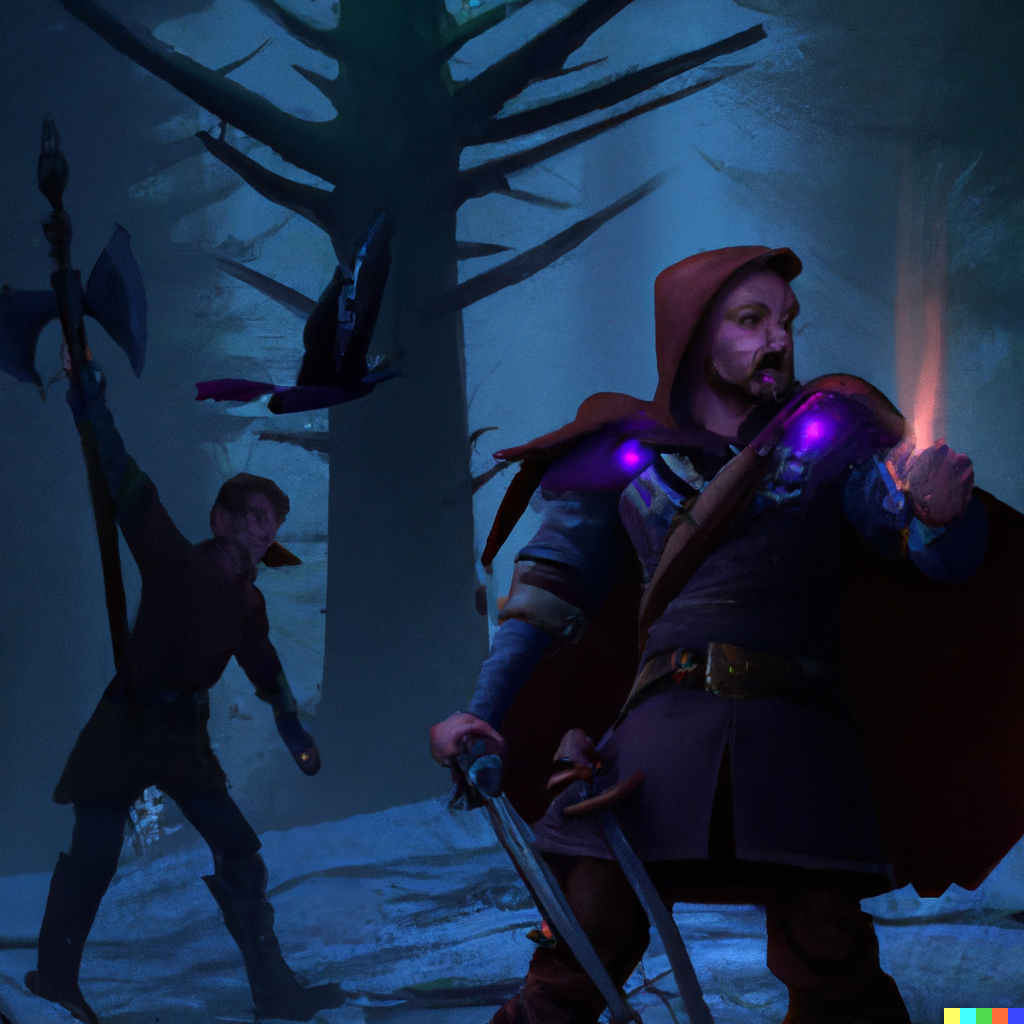
\includegraphics[width=\columnwidth]{combat/vision and light}

    Some creatures have \trait{darkvision} or other extraordinary senses, but most creatures need light to see by. 
    In an area of \glossterm{bright illumination}, all characters can see clearly.

    Creatures can see only dimly into areas that have \glossterm{shadowy illumination}.
    Everything in the area has \glossterm{concealment}.
    This allows creatures in the area to make Stealth checks to hide even if they don't have \glossterm{cover} (see \pcref{Stealth}).

    In an area with \glossterm{brilliant illumination}, creatures can see clearly just like an area with bright illumination.
    In addition, no shadows exist within an an area of brilliant illumination.
    This makes many effects from the \sphere{umbramancy} mystic sphere difficult or impossible to use.

    In areas of total darkness, creatures without \trait{darkvision} or some other form of supernatural vision are \blinded.

    \subsection{Attacking Unseen Foes}
        You can make \glossterm{targeted} attacks against creatures and objects you cannot see.
        To do so, you choose a 5-foot square and make the attack against that square.
        You have a 50\% \glossterm{miss chance} with the attack.
        Otherwise, you hit a random valid target in that square with your attack, if one exists.

    \subsection{Concealment}\label{Concealment}
        Concealment represents anything which makes it more difficult to see your target, such as \glossterm{shadowy illumination}.
        All \glossterm{targeted} attacks against a creature or object with concealment from you have a 20\% \glossterm{miss chance}.
        Generally, this means that you roll 1d10, and the attack misses on a 1 or 2.
        Determining concealment works similarly to determining cover.
        You must use the same \glossterm{points of origin} and \glossterm{target square} when determining concealment that you would use to determine cover.

        \parhead{Determining Concealment} There are two things that can cause a creature to be concealed: poor lighting, and intervening obstacles that block sight.
        Determining concealment from obstacles that block sight works the same way as determining cover (see \pcref{Cover}).

        Determining concealment from lighting conditions is simpler, since it ignores lighting conditions between you and the target.
        If your \glossterm{target square} is in lighting that provides concealment, the target has concealment.
        Otherwise, it does not.

\section{Obstacles and Cover}\label{Obstacles and Cover}
    In a battle, you may not be able to perfectly see all of your opponents.
    When obstacles get in the way, they may make some attacks impossible.
    Almost all abilities, including \glossterm{strikes}, must have \glossterm{line of sight} and \glossterm{line of effect}.
    Smaller obstacles may simply provide \glossterm{cover} instead of making attacks impossible.
    This section explains how to deal with obstacles and related limitations.

    \subsection{Point of Origin}\label{Point of Origin}
        When you make an attack, you have to determine the \glossterm{point of origin}.
        For \glossterm{targeted} attacks, which are the most common, the point or origin is a grid intersection of your choice that is touching your \glossterm{space}.
        For area attacks, the point of origin depends on the shape of the area and whether it has a defined \glossterm{range}.

        If an area attack has a defined range, the point of origin is a single grid intersection of your choice within that range.
        Cones, lines, and walls without a range use a grid intersection of your choice that is touching your space, just like targeted attacks.
        Cylinders and spheres without a range are unusual, since they radiate from your whole body instead of a single point.
        When determining their total size, treat every grid intersection touching your space as a point of origin.
        When determining cover and similar effects, only use the grid intersection that is closest to the target.

    \subsection{Cover}\label{Cover}

        Cover represents any obstacle that physically prevents you from striking your target, such as a tree or intervening creature.
        A creature or object behind cover gains a \plus2 bonus to Armor and Reflex defenses.
        If an attack misses the defense of a creature or object behind cover by no more than the defense bonus provided by the cover,
            the attack is applied to the obstacle instead of to the intended target.
        In the case of area attacks, this cannot cause an individual creature or object to be targeted or attacked twice by the same ability.
        This can protect creatures behind cover from \glossterm{glancing blows} (see \pcref{Glancing Blows}).
        In addition, a creature behind cover can hide (see \pcref{Stealth}).

        Cover is only relevant if the attacker has \glossterm{line of effect} to its target (see \pcref{Line of Effect}).
        If you don't have line of effect, you generally can't attack the target at all, so the defense bonuses from cover don't matter.

        \subsubsection{Measuring Cover}
            To measure cover for a particular attack, draw a cone from the attack's point of origin to the two closest corners of the target's space.
            Note that these must be corners where the target's space ends, not just grid intersections touching the target's space.
            The defender can choose between equally distant corners.
            If there are any obstacles in that cone, the target has cover.

            Obstacles only provide cover if the relevant part of the obstacle is no more than one size category smaller than the target.
            You should ignore any irrelevant parts of the obstacle that are outside of the cone.
            For example, although a tree might be Gargantuan or Colossal if you include all of its leaves and branches, most trees are only a Medium size obstacle at ground level, since only their trunk is relevant.
            The rules typically ignore the complexity of three-dimensional space, so you'll have to estimate what would provide reasonable cover in some cases.

            \subsubsection{Improved Cover}
            Cover of the same type generally doesn't stack; a creature behind two trees is not substantially more protected than a creature behind a single tree.
            However, exceptionally well covered creatures, such as a creature behind an arrow slit in a castle, may gain a greater than normal benefit to defenses from cover at the GM's discretion.

    \subsection{Line of Sight}\label{Line of Sight}
        Unless otherwise noted in an ability's description, you cannot target a creature, object, or location that you do not have line of sight to.
        Line of sight measures whether you can see things, not whether you can touch or reach them.

        A line of sight is a straight, unblocked path between an attacker and a target.
        To measure line of sight for a particular attack, draw a line between any grid intersection touching your \glossterm{space} and any grid intersection touching the target's space.
        If you're targeting a particular point, you would naturally draw the line to that point instead.
        If this line is not blocked by any obstacles that impede sight, you have line of sight to your target.

    \subsection{Line of Effect}\label{Line of Effect}
        Almost all abilities, including \glossterm{strikes}, must have a \glossterm{line of effect} to function.
        Line of effect measures whether physical passage is possible between two locations, regardless of any sight obstacles.
        For example, a pane of glass would block line of effect, but not line of sight.

        Unless otherwise noted in an ability's description, you cannot target a creature, object, or location that you do not have line of effect to.
        In addition, abilities that affect an area do not affect targets that the ability does not have line of effect to.

        A line of effect is a straight, unblocked path between an attacker and a target.
        To measure line of sight for a particular attack, draw a line between the attack's \glossterm{point of origin} and any grid intersection touching the target's space.
        If you're targeting a particular point, you would naturally draw the line to that point instead.
        If this line is not blocked by any obstacles that make physical passage impossible, you have line of effect to your target.

        \subsubsection{Destroying Barriers}\label{Destroying Barriers}
            Some abilities deal damage to both creatures and objects.
            If a physical barrier is \glossterm{broken} by an ability, that barrier does not affect the ability's line of effect.
            For example, a thin curtain of silk normally blocks line of effect.
            However, an ability that destroyed the curtain would have its full effect on everything behind the curtain.

        \subsubsection{Inside Creatures}
            Creatures block line of effect to the inside of their own bodies.
            As a result, you cannot use an ability that takes effect inside a creature unless you are also inside the creature.
            This restriction applies even if there is no physical barrier to the inside of the creature.
            For example, you cannot place the \glossterm{point of origin} for an area inside a creature's mouth, even if the creature has its mouth open at the time.

\section{Awareness and Surprise}\label{Awareness and Surprise}
    In combat, creatures are sometimes not fully aware of danger, which makes them less able to defend against it.
    A creature can be described as either aware, \unaware, or \partiallyunaware of an attack against it.
    Normally, creatures are aware of all attacks against them in combat.
    This causes no special bonuses or penalties.

    Sometimes, creatures are fully \unaware that they are in danger from attack.
    This typically happens as a result of stealth, but it can also happen as a result of sudden treachery.
    A creature takes a \minus5 penalty to Armor and Reflex defenses against attacks that it is unaware of.
    After being attacked, an unaware creature typically stops being fully unaware of future attacks.

    A creature that knows that it is in danger and is attempting to defend itself, but does not know the exact location or nature of its attackers, is \partiallyunaware.
    For example, a creature that is already in combat that is attacked by a previously unseen foe is partially unaware of the attack.
    Similarly, a creature that just barely fails to beat an opponent's Stealth check may hear an ominous sound that makes it partially aware of danger without knowing the exact location of any attackers.

    \subsection{Surprise Attacks}\label{Surprise Attacks}
        Sometimes, creatures are not aware that combat is taking place when the combat starts.
        This most commonly happens with ambushes.
        Any creature that is not aware of the combat continues taking whatever actions it would normally be taking until it becomes aware of the combat.
        It is usually \unaware of all until that point, though unusually vigilant or perceptive creatures may be \partiallyunaware.

        If a surprise attack begins a combat, the creatures who initiate the attack can choose which phase to start in.
        Generally, they should start in \glossterm{action phase}, though sometimes the \glossterm{movement phase} is more advantageous for the attackers.

\section{Poison}\label{Poison}
    Poisons can deal damage, weaken creatures, or even kill them.
    Some effects which are not literally poisonous, such as animal venom or fungal spores, are considered poisons.
    Unless otherwise noted, poisons are not \glossterm{conditions}, and cannot be removed by abilities that remove conditions (see \pcref{Conditions}).
    Common poisons are listed in \tref{Consumable Tools}.

    \subsection{Poison Transmission}\label{Poison Transmission}\label{Transmission}

        There are three ways that poisons can be contracted.

        \parhead{Contact} A contact poison affects any creature that touches it with bare skin.
        \parhead{Ingestion} An ingestion poison affects any creature that eats, drinks, or breathes it, depending on the type of poison.
        Ingestion poisons have no effect when touched or used to coat weapons.
        \parhead{Injury} An injury poison affects any creature that loses \glossterm{hit points} from something bearing the poison.
        Almost all injury poisons take liquid form, and are typically used to coat weapons.

    \subsection{Poison Forms}\label{Poison Forms}

        There are four forms of poison.

        \parhead{Gas} Gaseous poisons are difficult to store, but easy to affect foes with.
        Unless otherwise noted, a gas poison can be thrown within \shortrange, and affects a \tinyarea radius.
        \parhead{Liquid} Liquid poisons are the most common type of poison.
        Liquid poisons can be used to coat weapons, slipped into food, or simply thrown at foes.
        A dose of a liquid poison is usually about one ounce of the poison.
        \parhead{Pellet} Some rare poisons come in small, solid pellets or cubes.
        Typically, these pellets contain a powerful liquid poison that becomes inert quickly after being exposed.
        Pellet poisons are typically applied by being slipped into food.
        \parhead{Powder} Poison in powder form cannot be used to coat weapons, but can be slipped into food or thrown at foes.
        Unless otherwise noted, a powder poison functions as a \glossterm{thrown weapon} with \glossterm{range limits} of 5/15.

    \subsection{Coating Weapons with Poison}\label{Coating Weapons with Poison}
        As a standard action, you can coat a weapon with a single dose of a liquid contact-based or injury-based poison.
        The next time a creature takes damage from a \glossterm{strike} using that weapon, the struck creature is affected by the poison.
        This removes one dose of the poison from the weapon.
        Coated poisons expire and lose their effectiveness after ten minutes.

        Strikes that do not deal damage do not remove poison doses from a poisoned weapon.
        An injury-based poison has no effect if the strike does not cause the struck creature to lose \glossterm{hit points}, but the dose is still removed from the weapon.
        For this reason, injury-based poisons are typically applied to secondary weapons that can be used after the subject is already weakened.

        A weapon can hold up to three poison doses of the same poison.
        Mixing different poison types on the same weapon is ineffective, as each poison dilutes the others.
        Only the highest rank poison on the weapon has any effect.
        Choose randomly between equal rank poisons to determine which poison remains effective.

    \subsection{Poison Effects}\label{Poison Effects}

        Poisons can have a wide variety of effects, as determined by the type of poison used.
        However, most poison share certain common properties.

        \parhead{Becoming Poisoned}
        All poisons have an base \glossterm{accuracy}.
        When a creature first comes into contact with a poison, the poison makes an attack roll using its accuracy against the Fortitude defense of the poisoned creature.
        On a hit, the target becomes \glossterm{poisoned} and suffers the effects of the first stage of the poison.
        On a critical hit, the target becomes \glossterm{poisoned} and suffers the effects of the two stages of the poison.
        On a miss, the target is not \glossterm{poisoned}.

        Some attacks make the target poisoned if they hit the target.
        In that case, the ability's accuracy defines the poison's accuracy.

        Many poisons have an additional effect when they hit the target for the third time.

        \parhead{Poison Attacks}
        During each subsequent \glossterm{action phase} after the target becomes poisoned, the poison makes an attack roll against the Fortitude defense of the poisoned creature.
        If the poison was applied by a spell or other special ability, the accuracy bonus of this attack is equal to the accuracy of the original ability that applied the poison.

        Each hit increases the \glossterm{poison stage} of the poison.
        For every 10 points by which the attack hits, the poison progresses by an additional stage.
        On a miss, the creature gets closer to resisting the poison (see Resisting Poisons, below).

        \parhead{Resisting Poisons}
        If a poison misses a creature three times with its attack during each action phase, the creature stops being poisoned by that poison.
        % Some poisons may require more attacks to end the poison, as indicated in their description.

        \parhead{Multiple Doses}
        A creature can be affected by multiple doses of the same poison.
        This does not cause the same effect to occur multiple times.
        However, each extra dose increases the accuracy of the poison by 1, up to a maximum bonus of \plus10 more than the poison's normal accuracy.

        A poison is considered the same if it has the same name and comes from the same source.
        For example, a creature bitten multiple times by the same giant spider suffers multiple doses of the same poison.
        A creature bitten multiple times by different giant spiders considers each spider's poison separately.

        \parhead{Poison Quality} Some poisons are unusually high or low quality.

    \subsection{Creating Poisons}\label{Creating Poisons}

        You can use the Craft (poison) skill to create poisons.
        To create a poison, you must make a Craft (poison) check against a \glossterm{difficulty value} equal to 10 \add the poison's base accuracy.
        For every 2 points by which you beat this \glossterm{difficulty value}, the created poison's accuracy gains a \plus1 bonus, up to a maximum bonus of \plus10 more than the poison's base accuracy.

        Creating a poison requires special materials.
        The type of materials required, and how those materials can be acquired, depend on the type of poison.

        \begin{itemize}
            \itemhead{Plant} Plant-based poisons can typically be harvested by making a Survival check to search in appropriate terrain.
                The \glossterm{difficulty value} of this check is usually equal to 10 \add the base accuracy of the poison.
            \itemhead{Venom} Venom requires an appropriate body part from a creature -- often, poison it naturally produces.
            \itemhead{Alchemical} Alchemical poisons require alchemical materials.
                These cannot normally be found in nature.
                In unusual circumstances, these components can be synthesized from natural chemicals or magical materials with a Craft (alchemy) check equal to 10 \add the base accuracy of the poison.
        \end{itemize}

% TODO: This is a bad name; organize these better
\section{Special Combat Rules}

    \subsection{Mounted Combat}\label{Mounted Combat}
        \parhead{Horses in Combat} Warhorses and warponies can serve readily as combat steeds. Light horses, ponies, and heavy horses, however, are frightened by combat.
        At the start of each round, you must make a \glossterm{difficulty value} 10 Ride check to control such a horse.
        Success means you can act normally that round, directing the horse's movements as if it was trained for combat.
        Failure means that the horse acts of its own volition that round, usually fleeing in panic.

        \parhead{Space} A horse (not a pony) is a Large creature, and thus takes up a space 10 feet (2 squares) across. While mounted, you share your mount's space completely. Anyone who is close enough to hit your mount can attack either you or your mount.

        In the case of abnormally large mounts (two or more size categories larger than you), you may not completely share space. Such situations should be handled on a case-by-case basis, depending on the nature of the mount.

        \parhead{Flying Mounts} Flying mounts are harder to ride and control than terrestrial mounts, especially mounts that can change directions rapidly.
        The \glossterm{difficulty value} for all Ride checks on a mount using a fly speed is increased by 10 if the mount has poor or average maneuverability, or by 15 if it has perfect maneuverability.

        \parhead{Combat while Mounted} With a \glossterm{difficulty value} 5 Ride check, you can guide your mount with your knees so as to use both hands to attack or defend yourself. This is a free action.

        If your mount is moving in the current phase, you take a \minus2 accuracy penalty with ranged strikes.
        If your mount uses the \textit{sprint} ability, this penalty increases to \minus4 (see \pcref{Sprint}).

        \parhead{If Your Mount Falls in Battle} If your mount falls, you fall to the ground with it.

        \parhead{If You Are Dropped} If you are knocked unconscious, you fall from your mount to the ground, which may cause you to take \glossterm{falling damage}.
        If you have a military saddle, you stay on your mount instead.
        In either case, the mount acts according to its nature.
        Most mounts flee combat without a rider.

    \subsection{Allies and Enemies}\label{Allies and Enemies}
        Each creature you interact with in Rise is either an \glossterm{ally}, an \glossterm{enemy}, or a \glossterm{neutral party}.
        Some beneficial abilities only affect allies, and some offensive abilities only affect enemies.

        You can choose how you consider each creature at the start of each \glossterm{phase}.
        You cannot consider yourself an \glossterm{ally} or an \glossterm{enemy}.
        While you are \unconscious, you treat all creatures as \glossterm{allies}.

        \parhead{Allies} An ally is any creature you consider an ally who also considers you an ally.
        If you consider someone an ally, but they do not consider you an ally, you treat them as a neutral party for the purpose of your abilities.
        Allies can move through your \glossterm{space}.

        \parhead{Enemies} An enemy is any creature who you consider to be an enemy.
        Enemies cannot move through your \glossterm{space}.

        \parhead{Neutral Parties} A neutral party is any creature who is neither an ally nor an enemy.
        You treat all creatures you have not declared an opinion of as neutral parties.
        Neutral parties can move through your \glossterm{space}.

    \subsection{Teleportation}\label{Teleportation}
        Some abilities can \glossterm{teleport} creatures or objects.
        When you are teleported, you move through the Astral Plane and arrive at a new location.
        You can be teleported between two different locations on the same \glossterm{plane}, or between two different locations on different planes.
        If for some reason you cannot access the Astral Plane, you cannot be teleported.

        Unless an ability explicitly teleports to other planes or specifies otherwise, anything being teleported must have both \glossterm{line of sight} and \glossterm{line of effect} to its destination.
        Otherwise, the teleportation fails without effect.

        \subsubsection{Teleportation Noise}\label{Teleportation Noise}
            Creatures and objects that are teleported make a sound when they depart and arrive.
            This noise is caused by the displacement of air (or other substances) created by the teleportation.
            The base \glossterm{difficulty value} of an Awareness check to hear this sound for a Medium creature or object is 10.
            This difficulty value changes based on the size of the teleported creature or object:

            \begin{itemize}
                \item Fine: 30
                \item Diminutive: 25
                \item Tiny: 20
                \item Small: 15
                \item Medium: 10
                \item Large: 5
                \item Huge: 0
                \item Gargantuan: \minus5
                \item Colossal: \minus10
            \end{itemize}

        \subsubsection{Carrying Objects}
            When a creature is teleported, it can bring along equipment and held objects as long as two conditions are met.
            First, the combined weight of the objects cannot exceed the creature's maximum \glossterm{carrying capacity} (see \pcref{Weight Limits}).
            If a creature is teleported while carrying more than its maximum carrying capacity, all excess objects are left behind, starting with the heaviest object and proceeding in order of weight.

            Second, no object can extend more than two feet away from the creature's body.
            Any objects that extend beyond that distance are left behind.
            For example, a creature wearing handcuffs will arrive at its teleportation destination still wearing the handcuffs.
            However, a creature that is tied to a post by a long rope will arrive at its teleportation destination without the rope.

        \subsubsection{Horizontal Teleportation}
            Some planes have a curved primary surface.
            On those planes, ``horizontal'' teleportation isn't objectively horizontal.
            Instead, it is horizontal relative to the surface of the plane.
